Previous studies of LFU in $b\to sl^+l^-$ decays have indicated a $\num{3.1}\sigma$ 
deviation from the predictions of the Standard Model \cite{previous_RK}, \cite{previous_RK*}. 
Similar deviations have been observed in measurements of angular observables \cite{angular_1}, 
\cite{angular_2}. This proceeding discusses the first simultaneous measurement of electron-muon 
universality in the non-resonant regions of the decays $B^+\to K^+l^+l^-$ and $B^0\to K^{*0}l^+l^-$.

The observable $R$, which is used to test LFU, is defined as
\begin{equation}
    R_{K,K^*}= 
    \frac{\int_{q_a^2}^{q_b^2}\frac{\mathrm{d}\Gamma(B^{(+,0)}\to K^{(+,*0)}\mu^+\mu^-)}{\mathrm{d}q^2}\mathrm{d}q^2}
    {\int_{q_a^2}^{q_b^2}\frac{\mathrm{d}\Gamma(B^{(+,0)}\to K^{(+,*0)}e^+e^-)}{\mathrm{d}q^2}\mathrm{d}q^2} .
    \label{eqn:single_ratio}
\end{equation}

Theoretically, this ratio is predicted to be $\num{1}$, with corrections at 
the percent level \cite{LU_theo}. 
As the decay is depending on the dileptonmass $q^2$, the dataset is divided into four $q^2$ regions:
a non-resonant low $q^2$ region ranging from
$\SIrange{0.1}{1.1}{\giga\electronvolt\squared}$,
a non-resonant central region ranging from
$\SIrange{1.1}{6.0}{\giga\electronvolt\squared}$,
and the regions for the $J/\Psi$ resonance ranging from 
$\SIrange{6.0}{11}{\giga\electronvolt\squared}$
and for the $\Psi(2S)$ resonance ranging from
$\SIrange{11}{15}{\giga\electronvolt\squared}$.

To mitigate uncertainties arising from efficiencies, the double ratio 
\begin{equation}
    R_{K,K^*}= 
    \frac{\frac{N}{\epsilon}(B^{(+,0)}\to K^{(+,*0)}\mu^+\mu^-)}
    {\frac{N}{\epsilon}(B^{(+,0)}\to K^{(+,*0)}e^+e^-)}
    \underbrace{\frac{\frac{N}{\epsilon}(J/\Psi(e^+e^-))}{\frac{N}{\epsilon}(J/\Psi(\mu^+\mu^-))}}_{(r^K_{J/\Psi})^{-1}}
    \label{eqn:double_ratio}
\end{equation}
is defined.

In this equation, $N/\epsilon$ represents the yield of the process, corrected by 
the efficiency. The resonant part, $r^K_{J/\Psi}$, is known to be $\num{1}$ 
\cite{AULCHENKO2014227}. Due to the complexity involved in estimating efficiencies, 
the double ratio provides a more stable measure against systematic uncertainties.

The Large Hadron Collider beauty experiment (LHCb) is one of the four major experiments 
at the Large Hadron Collider (LHC) at CERN. It is designed to conduct high-precision 
measurements of particle decays involving b and c quarks. Given that $b\bar{b}$ pairs 
are boosted in the beam direction, the detector is constructed as a single-arm forward 
spectrometer \cite{LHCb}.

The LHCb trigger system is a three-level system designed to select relevant events from 
the multitude of proton-proton collisions. The first level, known as the Level-0 trigger 
(L0), is hardware-based and reduces the event rate based on information from the calorimeter 
and muon systems. The subsequent levels, HLT1 and HLT2, are software-based. HLT1 applies 
fundamental conditions for partially reconstructed events, while HLT2 utilizes complete 
reconstruction of candidates and employs topological information to further reduce the 
data volume \cite{trigger}.

Particle identification (PID) at LHCb is carried out using information from several 
sub-detectors. The RICH (Ring Imaging Cherenkov) detectors provide PID information by 
measuring the Cherenkov angle of charged particles. The calorimeter system is utilized 
to identify photons, electrons, and hadrons, and to measure their energies. The muon 
system is employed to identify muons. The performance of the PID system is crucial for 
numerous analyses at LHCb, including the measurement of lepton universality in $b\to sll$ 
decays.

The reconstruction of decay in the electron and muon channels presents varying levels of complexity, 
primarily due to three factors. Electrons emit bremsstrahlung, which adds a layer of complexity to the 
reconstruction process. Additionally, the electronic calorimeter's energy resolution is characterized 
by substantial uncertainties. Last the efficiencies of the L0 triggers for muons and electrons 
differ. These elements contribute to differences in the efficiencies in 
the two channels. 

To neutralize the varying efficiencies of the L0 trigger, one can employ events that are 
triggered independently of the signal, known as Trigger Independent Signal (TIS) events. 
In these instances, the $B$ candidate does not influence the trigger, thereby ensuring that 
the efficiencies between the electron and muon modes are balanced.

%The simulations are generated for each period of datataking via 

To enhance the signal-to-background ratio, two multivariate classifiers are employed. The 
first classifier is designed to distinguish the signal from the combinatorial background, 
which is composed of randomly assembled tracks. This classifier utilizes information about 
the kinematics and geometry of the final state, as well as details about the vertex and the 
quality of the vertex fit.

The second classifier is used to differentiate between the signal and partially reconstructed 
background. These are processes with additional particles $X$ in the final states, such as 
$B\to K l^+l^- X$. If particle $X$ is not correctly reconstructed, the process may be mistakenly 
identified as $B \to K l^+l^-$. This classifier also uses kinematic and geometric features of 
the final states, but additionally, it incorporates information about the spatial and kinematic 
isolation of the final state particles in relation to other reconstructed particles.

To avoid bias, a $k$-folding validation is implemented. Both classifiers are optimized 
simultaneously for each lepton flavor, $q^2$ region, and data-taking period separatly.

% ab hier wirds kompliziert :(

The simulations utilized in the analysis are calibrated to accurately represent the difference 
between electrons and muons. To achieve this, weights are computed via 
$w_i=\epsilon_\text{data}/\epsilon_{Simulation}$ for the $J/\Psi$ resonant decaysin a chain 
for each calibration category $i$. 

The effects of these corrections are illustrated in Figure \ref{fig:weights}. 
It is evident that the double ratios $R$ are significantly less influenced by the corrections 
than the single ratio $r^{K^*}_{J/\Psi}$. The single ratio efficiency changes by $\SI{25}{\%}$, 
while all double ratio efficiencies are altered by at most $\SI{5}{\%}$. This demonstrates that 
the double ratio is a more robust observable than the single ratio when it comes to uncertainties 
in the efficiencies.

\begin{figure}
    \centering
    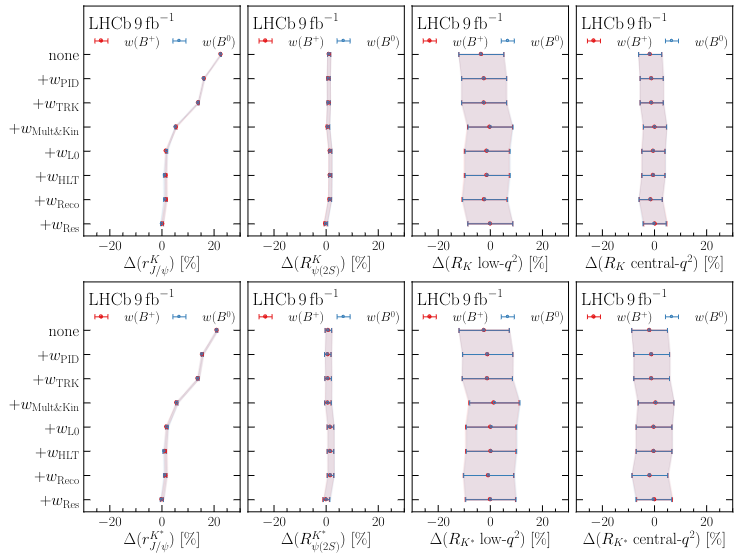
\includegraphics[width=\linewidth]{figures/weights.png}
    \caption{Variation of the efficiencies regarding to the corrections for all four $q^2$ ranges \cite{lhcbcollaboration2022test}.}
    \label{fig:weights}
\end{figure}
To crosscheck all previous steps $r^{K^{(*)}}_{J/\Psi}$ and $R^{K^{(*)}}_{\Psi(2S)}$ are 
calculated. As expected all of them are compatible with $\num{1}$.

The calculation of the doubleratio is done by a simultaneous maximum-likelihood fit 
of the invariant mass distribution of the reconstructed $B^0$ and $B^+$ in the non
resonant $q^2$ regions and the $J/\Psi$ resonance. 

The invariant mass distribution in the muon mode only consits of the signal an 
combinatorial background.
In the case of the electron, the distribution is much more complicated due to 
residual missidentified hadronic decays and partially reconstructed backgorund. 
Additionally there are contributions of the resonant $J/\Psi$ decay that reach 
into the central $q^2$ region.
The shapes of the signal, misidentified, and partially reconstructed backgrounds 
are determined from the simulations. The combinatorial background is modeld as a 
decreasing exponential function. 
The signalyield is then used to calculate the doubleratio using \eqref{eqn:double_ratio}.
\begin{figure}
    \centering
    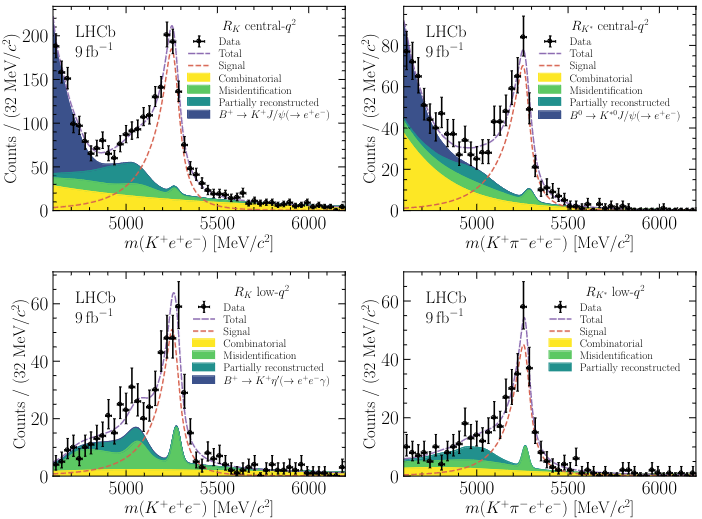
\includegraphics[width=\linewidth]{figures/fits.png}
    \caption{Maximum likelihood fit of the invariant mass distributions in the central $q^2$ (upper) and lower $q^2$ (lower) for the non-resonant decays $B^+\to K^+e^+e^-$ (left) and $B^0\to K^{*0}e^+e^-$ (right) \cite{lhcbcollaboration2022test}.}
    \label{fig:fits}
\end{figure}

The obtained results for the observalbles yield the outcomes
\begin{align*}
    \text{low $q^2$:} 
    &\left\{
    \begin{aligned}
        &R_{K}  \!\!\!\!\!\!\!&&=\, 0.994 \,\substack{+0.090 \\ -0.082}\,\text{(stat)}\,\substack{+0.029 \\ -0.027}\,\text{(syst)}\\
        &R_{K^*}\!\!\!\!\!\!\!&&=\, 0.927 \,\substack{+0.093 \\ -0.087}\,\text{(stat)}\,\substack{+0.036 \\ -0.035}\,\text{(syst)}
    \end{aligned}
    \right. \\
    \text{central $q^2$:} 
    &\left\{
    \begin{aligned}
        &R_{K}  \!\!\!\!\!\!\!&&=\, 0.949 \,\substack{+0.042 \\ -0.041}\,\text{(stat)}\,\substack{+0.022 \\ -0.022}\,\text{(syst)}\\
        &R_{K^*}\!\!\!\!\!\!\!&&=\, 1.027 \,\substack{+0.072 \\ -0.068}\,\text{(stat)}\,\substack{+0.027 \\ -0.026}\,\text{(syst)}.
    \end{aligned}
    \right.
\end{align*}

The dominant sources of systematic uncertainty in the modeling of 
invariant mass distributions arise from the data-driven modeling 
of misidentified backgrounds. These uncertainties vary from 
$\SI{2.0}{\%}$ to $\SI{2.5}{\%}$, depending on the specific observable. 
Another significant source of uncertainty is associated with the 
stability of the single ratios $r^{K^{(*)}}_{J/\Psi}$, which depends on 
the kinematics and geometry of the decay. However, excluding the low 
$q^2$ region for $R_{K^*}$, this uncertainty contributes significantly 
less than the uncertainty stemming from the modeling of misidentified 
backgrounds. Overall, the statistical uncertainties dominate the total 
uncertainty of the results.